% A Discussion of Data Science in Healthcare
% Jacob Sánchez Pérez (jacob@san.contact)
% Data Science (CO3722)
% University of Central Lancashire

\documentclass[a4paper,11pt]{article}

% Links
\usepackage{hyperref}

% PDF Metadata
\hypersetup{
    hidelinks,
    pdftitle={A Discussion of Data Science in Healthcare},
    pdfauthor={Jacob Sánchez}
}

% Code
\usepackage{minted}

% Referencing and more
\usepackage[british]{babel}
\usepackage{csquotes}
\usepackage[style=apa,backend=biber]{biblatex}

% Images
\usepackage{graphicx}
\graphicspath{ {./figures/} }

% Graphs
\usepackage{pgfplots}
\pgfplotsset{width=10cm,compat=1.9}
\usepgfplotslibrary{external}
\tikzexternalize

\title{A Discussion of Data Science in Healthcare to Identify Disease Risk Factors}
\author{Jacob Sánchez Pérez\\ University of Central Lancashire\\\texttt{jsanchez-perez@uclan.ac.uk}}
\date{}

\addbibresource{references.bib}

\begin{document}

\maketitle


\section{Introduction}

% PROMPT
% This section will introduce your project, your business, specific Use Case and potential source of a dataset for analysis.

% NOTES
% The business I have chosen is healthcare

Data science applies different methods in order to solve relevant problems and
make predictions \parencite[78]{Waller2013}.
One industry that can benefit from data science is the healthcare industry.
By improving productivity, public spending can be significantly reduced \parencite{oecd2010health}.
McKinsey estimated that data analytics can reduce healthcare expenses by up to
\$450 billion annually in the U.S.\parencite{Groves2013}.
Data science can be used to process the massive amounts of electronic health
records that exist, including physician notes, medical records, patient scans,
and patient sensor data \parencite{Adam2017, Dalianis2015}.
Areas in healthcare that could have the most impact include early detection of
diseases, precision medicine, optimisation of workflows, value-based healthcare,
infection prevention and control, and clinical research \parencite[9]{Consoli2019}.

This report is centred around the application of data science to identify early
risk factors of diseases.
Prompt identification of risk factors of fatal diseases can be quite beneficial
to the healthcare industry.
For instance, Coronary Heart Disease (CHD) was found to have a total annual
burden of £7.06 billion in the UK, the highest for any disease \parencite{Liu2002}.
This report will review in detail the process of data analysis, from locating a
data source, processing the data, and finally visualising and interpreting the results.

\section{Discussion of Data Science for Healthcare}

% PROMPT
% This section will relate specifically to your business and Use Case and their approach or potential application for the use of data science.
% This will cover the challenge of acquiring or using specific data sources for your Use Case, approaches to data processing, description of proposed machine learning  algorithms and their design, opportunities for data visualisation and the methods for analysing/interpreting the data required to gain business competitive advantage.

\subsection{Challenges}

\subsubsection{Privacy Concerns}

The General Data Privacy Regulation (GDPR) in the E.U. and the Health Insurance
Portability and Accountability Act (HIPAA) in the U.S., protect data that can
identify a patient \parencite{Iyengar2018}.
GDPR requires explicit consent of the subject to process personal data.
Obtaining consent results impractical in big data analytics.
However, data can be processed for purposes such as research and analysis as
long as it is pseudonymised.
Pseudonymisation (de-identification) consists of replacing or removing direct
identifiers, such as names, phone numbers, and other identifying data \parencite{Hintze2018}.
Nowadays, de-identification can be performed through neural networks \parencite{Dernoncourt2016}.
However, no method is perfect and this is still a limiting factor in healthcare
data availability.

\subsubsection{Processing Concerns}

In addition to the legal issues, data processing can be a major obstacle.
In particular, clinical notes can contain misspelled words, medical jargon,
and non-standard words \parencite{Dalianis2015}.
Furthermore, data is oftentimes collected from systems with incompatible formats
\parencite[34]{Consoli2019}.
Therefore significant preprocessing will be necessary before analysing the data.

\subsection{Data Sourcing}

\subsubsection{Healthcare Data Sources}

A selection of anonymised datasets that are widely used in research due to
their relaxed access policy are listed in the Appendix
\ref{appendix:sources} \parencite{Dalianis2015}.

\subsubsection{Dataset Choice}

For the purpose of this report, the \textit{n2c2} dataset was chosen over the
other sources for its manageable size and ease of use.
Bigger datasets have the issue of becoming difficult to work with in consumer hardware,
since the records have to be pre-processed in a extensively to be able to use them.
Finally, the \textit{n2c2} datasets have the added benefit of being topic-focused,
which means that each dataset has been constructed with a particular health concern
or topic in mind.
From the different datasets contained in the \textit{n2c2} collection,
the one focusing in heart disease was selected, since heart disease is one of
the biggest public health concerns globally.
Additionally, there are several known risk factors for heart disease, which will
allow validation of the results \parencite{Kannel2002}.

The \textit{n2c2} heart disease dataset contains 1304 records which represent 296
diabetic patients \parencite{Kumar2015}.
After a request for access was filed and approved, the dataset was ready to be
analysed.


\subsection{Data Processing Techniques}

\subsubsection{De-identification}

De-identification techniques will not be covered here,
as the available datasets have been de-identified beforehand.
However, for the specific task of de-identification of the dataset in question,
\textcite{Yang2015} can be consulted (Figure \ref{fig:deid}).

% Kalman Filter Diagram
\begin{figure}[h]
\centering
\scriptsize
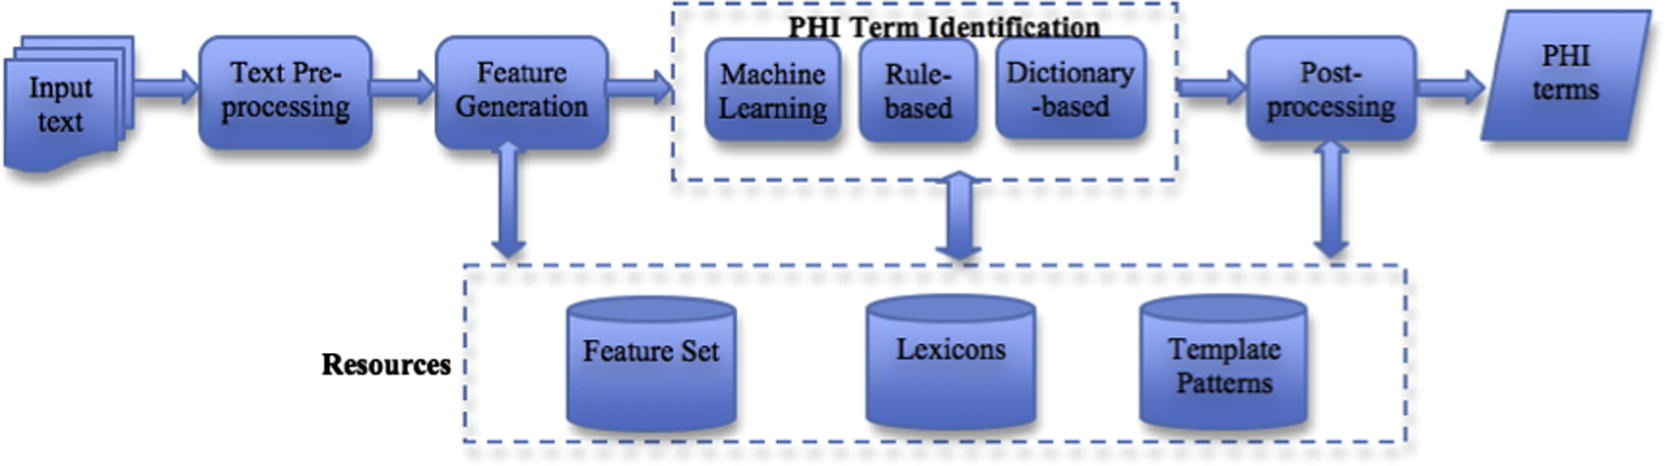
\includegraphics{deid}
\caption{De-identification Approach by \textcite{Yang2015}}
\label{fig:deid}
\end{figure}

\subsubsection{Data Cleaning}

Before performing any analysis, the integrity and quality of the dataset needs
to be assessed.
Missing values, misspellings, duplicates, and mixed formats can affect the
data quality \parencite{Chu2016}.
These present themselves as outliers, values that are more than two standard
deviations away from the mean.
Robust estimators, resampling, and exploratory data analysis are some ways to
detect them \parencite{Hellerstein2008}.
Additionally, categorical variables such as words or names that represent a
category or group can be handled by deduplication,
though there are alternatives such as encoding the similarity between
categories in the model itself \parencite{Cerda2018}.

\subsubsection{Text and Strings Specifics}

One of the most common ways to represent text in machine learning is a
\textit{bag-of-words}.
It stores every unique word in the text and the number of times it is mentioned.
Everything else (structure, formatting, and punctuation) is discarded.
Other techniques include \textit{stopwords} (discarding frequent words),
and \textit{term frequency–inverse document frequency}
(rescale features by their expected importance), n-grams,
stemming, and lemmatization, among others \parencite[327,344]{Mueller2017}.
In healthcare, some techniques that might improve the quality of free-text data
may include detection of negation and spelling mistakes, abbreviation normalisation,
and named entity recognition \parencite{Dalianis2015}.

\subsubsection{Dataset Processing}

In order to be able to apply machine learning algorithms to the \textit{n2c2}
dataset, the first step is to annotate the patient records.
This means processing the text and extracting the relevant features.
For instance, when the word \textquote{diabetes} occurs in a patient record,
the system should correctly identify this feature and label the record as such.
The \textit{n2c2} dataset provides pre-annotated training and test data.
However, some approaches work best with custom annotations, such as
\textcite{Roberts2014}, which manually annotated the heart disease dataset to
better suit their model design.

\subsection{Supervised Learning Algorithms}

A summary of different Machine Learning learning methods can be consulted in the
Appendix \ref{appendix:ml}.
\textcite{Jothi2015} outlined some of the supervised learning algorithms
commonly used in healthcare data analysis, briefly described next.

\begin{description}
    \item[Decision Tree] A hierarchy of if/else questions, that lead to a decision \parencite{Mueller2017}.
    \item[K-nearest Neighbour] Returns the closest point in the training dataset
    to make a prediction \parencite{Mueller2017}.
    \item[Logistic Regression] Statistical technique that makes binary decisions
    based on a logistic curve \parencite{Nick2007}.
    \item[Bayesian Classifier] Each feature is analysed individually, then,
    per-class statistics are collected for each feature. 
    To make predictions, the \textquote[{\cite[69]{Mueller2017}}]{data point is
    compared to the statistics for each of the classes,
    and the best matching class is predicted}.
    \item[Support Vector] Identifies those data points which exist between classes
    (the support vectors) and from them a decision boundary is defined.
    Classification is made based on the distances to the support vectors \parencite[98]{Mueller2017}.
\end{description}


Finally, Deep Learning encompasses several techniques that vary in complexity and design \parencite{Ibrahim2021}.
Some deep learning architectures are:

\begin{itemize}
 \item Convolutional Neural Networks (CNN)
 \item Recurrent Neural Networks (RNN)
 \item Deep auto-encoders
\end{itemize}

\subsubsection{Dataset Algorithms}

When considering the \textit{n2c2} dataset, it is necessary to ask the question
of which algorithms perform better for heart disease detection.
\textcite{Khan2019} surveyed 35 journal articles and found that the three most
popular techniques when classifying heart disease datasets are Support Vector
Machines, Neural Networks, and combined approaches.
However, popularity alone cannot justify the algorithm choice.
\textcite{Stubbs2015} reviewed the original most effective approaches to
classification of the heart disease \textit{n2c2} dataset.
All of the three most performant approaches (in terms of precision and recall)
used Support Vector Machines in combination with other methods such as manual
rules.
This findings would point towards a preference in using Support Vector Machines
as the main algorithm when analysing the dataset along with handcrafted rules.

\subsection{Training and Testing Approaches}

The training and testing strategy of a model can affect its accuracy.
\textcite[39]{Consoli2019} suggests using the \(k\)-fold cross-validation approach,
in which the dataset is split into \(k\) parts, of which \(k-1\) parts are used
to train the model, and one is used to test it, rotating the data such that
every part is used to test it once.
\textcite{Wong2020} suggested 10-fold cross validation to be the best first
approach, with less folds only being viable in small datasets.
\textit{Stratified k-fold cross-validation}, is a slight variation of this,
in which the data is split keeping adequate proportions of each class in each fold \parencite{Mueller2017}.
Since in the \textit{n2c2} dataset there are more than a thousand records,
10-fold cross validation is possible and recommended.

\subsection{Data Visualisation}

The way results are represented is important, since visualisations can make
patterns apparent and provide insights that can alter the final decision
\parencite{Hendriks2019}.
Transparency and lack of bias are desirable qualities in a visualisation
technique \parencite{Hendriks2019}.
Graphical representation can reveal features such as unusual distributions,
patterns, clusters, gaps, outliers, and much more \parencite{Unwin2020}.
Visualisation techniques can come in forms such as scatter plots, line graphs,
bar charts, histograms, and heat maps \parencite{Sadiku2016}.
Visualisation can be of help when analysing the heart disease dataset.
For instance, after annotation, bar charts can show the number of times certain
features appear in the dataset.
Furthermore, a scatter plot can be created to show the relation between certain
risk factors (such as age, cholesterol levels, and blood pressure) and the
likelihood of developing a heart condition.

\subsection{Model Interpretation}

In order to be useful in practice, a model in healthcare needs to be interpretable
by medical professionals, since they need to be able to make decisions based on
the behaviour of the model.
Interpretability is determined by the degree to which of humans
are able to understand its decisions and rationale.
One of the disadvantages of many machine learning models is their lack of
transparency, which makes interpretation a difficult task \parencite{Stiglic2020}.
Good interpretability results in a model that is fair, unbiased, privacy-oriented,
trustworthy, and reliable, values that are of upmost importance in healthcare \parencite{DoshiVelez2017}.

There are multiple criteria used to describe interpretability methods, based on
factors like the stage at which they are implemented, or whether they are
model-agnostic or model-specific.
Interpretability can be implemented at the data level (\textit{pre-model}),
at the model level (\textit{in-model}), or after the fact (\textit{post-model}).
Since it is of high priority in healthcare, interpretability should be part of
the model itself whenever possible (\textit{in-model}).
This would provide confidence that any decisions taken can be traced back and
explained to the patient, for example.


\section{Evaluation of Data Science in Healthcare}

% PROMPT
% You will evaluate the benefits or otherwise, including the challenges of
% applying machine learning algorithms, maintenance and ethical considerations
% of a data science model for business insight.
% ~400 words

\subsection{Impact of Data Science in Healthcare}


Data science is already being used in healthcare on a large scale, in areas from
administration to clinical decision support.
Advances that would otherwise be infeasible are now commonplace thanks to data
analysis.
However, data analytics still has many challenges and areas of opportunity.
For instance, \parencite{PeifferSmadja2020} found that ML clinical decision
support systems lacked quality and performance in clinical settings, and
highlighted opportunities such as data quantity and quality, interpretability,
and availability.


\subsection{Ethical Concerns}

More so than with other applications of data science, healthcare demands strict
ethical considerations and rules.
Many defend the position that data science in healthcare should be
heavily controlled by a solid and justified ethical framework \parencite{Baeroee2020}.
Failure to address ethical guidelines can result in biases in the model,
which could show up as unfair treatment of patients based on sex, race, or other.
These biases usually appear as a cause of biased training data.
Bias can occur when populations are underrepresented in the training data,
or when an existing systematic bias is replicated in the model \parencite{Chen2021}.
In contemporary applications of machine learning, bias is not difficult to find.
This is specially concerning with applications that can affect human life 
\parencite{Yapo2018}.

\subsection{Patient Privacy}

Some debate exists about the need for strict de-identification,
and how it can affect the availability of data.
\textcite[2]{Shin2018} argues that de-identification can lead to a distortion
and loss of detailed data, which can greatly impact the results of a study.
Likewise, \textcite{Kim2019} revealed that almost half (45.8\%) of all
participants in a survey thought that a revision in legislation was necessary
to reduce obstacles in healthcare data analysis.
However, it is important to remember that big data analytics can still have
consequences for individuals.
Some de-identification methods are vulnerable to correlation attacks, which can
identify individuals through indirect identifiers \parencite{Abouelmehdi2018}.
As \textcite{Abouelmehdi2018} points out, privacy agreements must be respected,
and sensitive information should remain private.


\section{Conclusions and Recommendations}

Data Science has advanced exponentially thanks to the advances in Machine
Learning and Artificial Intelligence of the last decades.
The literature about data analysis in healthcare is vast, and covers technical
areas such as sourcing, processing, cleaning, algorithms, deep learning,
visualisation, and much more.
This body of knowledge, along with current technology and tools make it
possible to imagine a future where hospitals, researchers, and scientists
harness their full potential.
However, privacy and consent should never be undermined for the sake of research,
and ethics should be a top priority when designing a machine learning approach.

\bigskip
Word count: 2200

% ~150 words
\pagebreak
\printbibliography

\pagebreak
\appendix

\section{Dataset Sources}\label{appendix:sources}

\paragraph{MIMIC-II} A collection of data from ICU patients,
spanning 7 years and ~27,000 patient admissions.
The dataset contains patient demographics, intravenous medication drip rates,
laboratory test results, and physiological waveforms recorded at bedside.
The dataset can be accessed after registration free of charge \parencite{Lee2011}.

\paragraph{MIMIC-III} A successor to \textit{MIMIC-II}, it spans more than a
decade and \textgreater 50k patient admissions.
It contains demographics, notes and reports, tests, along with bedside monitoring data.
As its predecessor, access merely requires registration \parencite{Johnson2016}.

\paragraph{THIN} It is an ongoing dataset which begins in 1994, and represents
6\% of the UK population.
It contains records from general practices.
The dataset can only be accessed by those with special authorisation,
such as research organisations \parencite{Lewis2007}.

\paragraph{n2c2} Formerly known as \textit{i2b2} , it is a collection of datasets
of topics including smoking, obesity, medication, and heart disease,
The dataset requires registration and access request approval, yet is free of cost.

\section{Machine Learning}\label{appendix:ml}

Machine learning algorithms can be classified by how they are trained:

\begin{itemize}
 \item Supervised Learning
 \item Unsupervised Learning
 \item Semisupervised Learning
 \item Reinforcement Learning
 \item Deep Learning
\end{itemize}

Supervised learning happens when the training data is labelled,
i.e. has been classified beforehand.
Unsupervised learning uses unlabelled data, which the model deduces a structure from.
In semisupervised learning, some data is labelled and other unlabelled.
Reinforcement learning conditions the model externally through feedback
\parencite[11]{Ibrahim2021}.
Lastly, deep learning involves a series of layers that process the data in series \parencite[13]{Ibrahim2021}.

\end{document}
